% LTex: language=pl
\section{Modyfikacja serwisu STOS}
By zwiększyć elastyczność systemu, proponujemy zmodyfikowanie obecnego interfejsu systemu STOS. Obecna implementacja funkcji komunikacji z serwisem, polega na porównaniu wartości otrzymanego nagłówka żądania do zdefiniowanego zestawu obsługiwanych komend i jego obsłudze. W przypadku potrzeby rozwoju należy rozwinąć instrukcję warunkową i dodać do niej obsługę nowego parametru oraz ustawić ten nagłówek w miejscu wysyłania żądania. Zwiększa to nieczytelność i trudność w utrzymaniu kodu. Ze względu na umieszczenie obsługi w bloku \textit{try-catch}, nie istnieje dedykowana obsługa błędu, co utrudnia diagnostykę w przypadku jego wystąpienia. Proponujemy stworzenie nowego interfejsu komunikacyjnego obsługującego żądania HTTP posiadającego trzy punkty końcowe:
\begin{itemize}
    \item Otrzymywanie metadanych zadania z kolejki -- punkt końcowy znajdujący się pod adresem \textit{/tasks}, wywoływany żądaniem typu \textit{GET}. Ma za zadanie zwrócić metadane zadania z kolejki i je usunąć. Zwracane dane będą zawierać identyfikatory plików testów, plików przesłanych przez studenta oraz zadania, które jest rozwiązywane. Usuwanie zadań z kolejki powinno być synchronizowane.
    \item Otrzymywanie pliku o określonym identyfikatorze -- punkt końcowy znajdujący się pod adresem \textit{/files/<id:int>}, wywoływany żądaniem typu GET. Zwraca plik oraz jego typ. Rozdział na możliwość pobierania pojedynczych pilików zamiast całego zestawu, pozwana na zastosowanie systemu pamięci podręcznej, która pozwoli na pominięcie kroku pobierania kilkukrotnie tego samego zbioru plików, szczególnie plików zawierających zadanie oraz testy, które w większości przypadków pozostają niezmienione.
    \item Zapisywanie wyniku zadania -- punkt końcowy znajdujący się pod adresem \textit{/tasks/<id:int>}, wywoływany żądaniem typu POST. Zapisuje wynik dla każdego z testów dla danego studenta, dla zadania określanego w żądaniu.
\end{itemize}
\newline \indent Każdy z punktów końcowych powinien być obsłużony w osobnej funkcji i posiadać odpowiednią obsługę wyjątków. Do implementacji sugerujemy użycie technologii PHP, Python, Java lub C# oraz opcjonalnie frameworków Laravel, Django, Flask, Spring lub ASP.NET. Sugerowane działanie zostało przedstawione na schemacie \ref{stos-suggestion}.
\begin{figure}[!h]
	\begin{center}
		\resizebox{1.0\textwidth}{!} {
			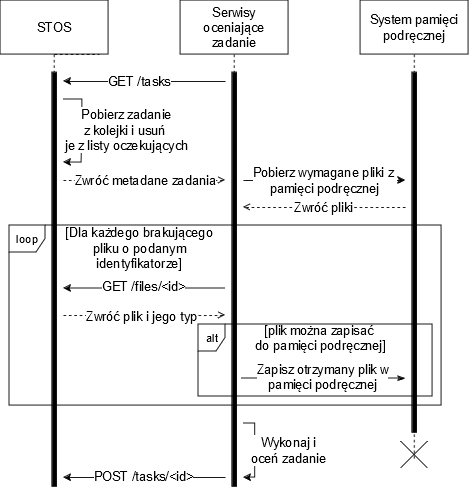
\includegraphics{img/5/stos-suggestion.png}
		}
		\caption[Schemat działania zaproponowanego serwisu. Źródło własne.]{Schemat działania zaproponowanego serwisu. Źródło własne.}
    \label{stos-suggestion}
	\end{center}
\end{figure}
